\section{Resoconto attività di verifica}
In tale sezione vengono descritti gli esiti delle attività di verifica svolte sui documenti redatti.

\subsection{Analisi dinamica dei documenti}
L'analisi dinamica mediante l'utilizzo dello strumento GitHub\ped{G} Actions\ped{G} ha garantito una stesura del codice \LaTeX{}\ped{G} priva di errori e più coesa fra tutti i membri del gruppo. Infatti, tramite questo strumento, è stato possibile individuare errori che potevano essere ignorati durante la compilazione locale del documento da qualche membro del team.

\subsection{Analisi statica dei documenti}
L'analisi statica dei documenti tramite \textit{Walkthrough}\ped{G} ha portato all'individuazione di errori comuni, i quali hanno portato ad un aggiornamento della lista di controllo già stilata in precedenza e consultabile all'interno delle \NdPv{} nella sezione \textit{Analisi statica}. In tale modo è stata resa più semplice e mirata l'attività di \textit{Inspection}\ped{G}. Inoltre sono stati riscontrati errori e/o migliorie per il template\ped{G} \LaTeX\ped{G} a cui fa riferimento ogni documento.

\subsection{Esiti delle verifiche dell'indice di Gulpease}
Di seguito è riportato il grafico dell'indice di Gulpease calcolato sui vari documenti, il cui valore è definito accettabile e ottimale come descritto nella sezione §2.2.1.1.\\
I dati fanno riferimento a:
\begin{itemize}
	\item \textbf{RR:} Revisione dei Requisiti;
	\item \textbf{RP:} Revisione di Progettazione;
	\item \textbf{RQ:} Revisione di Qualifica (da aggiungere con l'avanzare del progetto);
	\item \textbf{RA:} Revisione di Accettazione (da aggiungere con l'avanzare del progetto).
\end{itemize} 

\subsubsection{Grafico complessivo}

\begin{figure}[H]
\centering
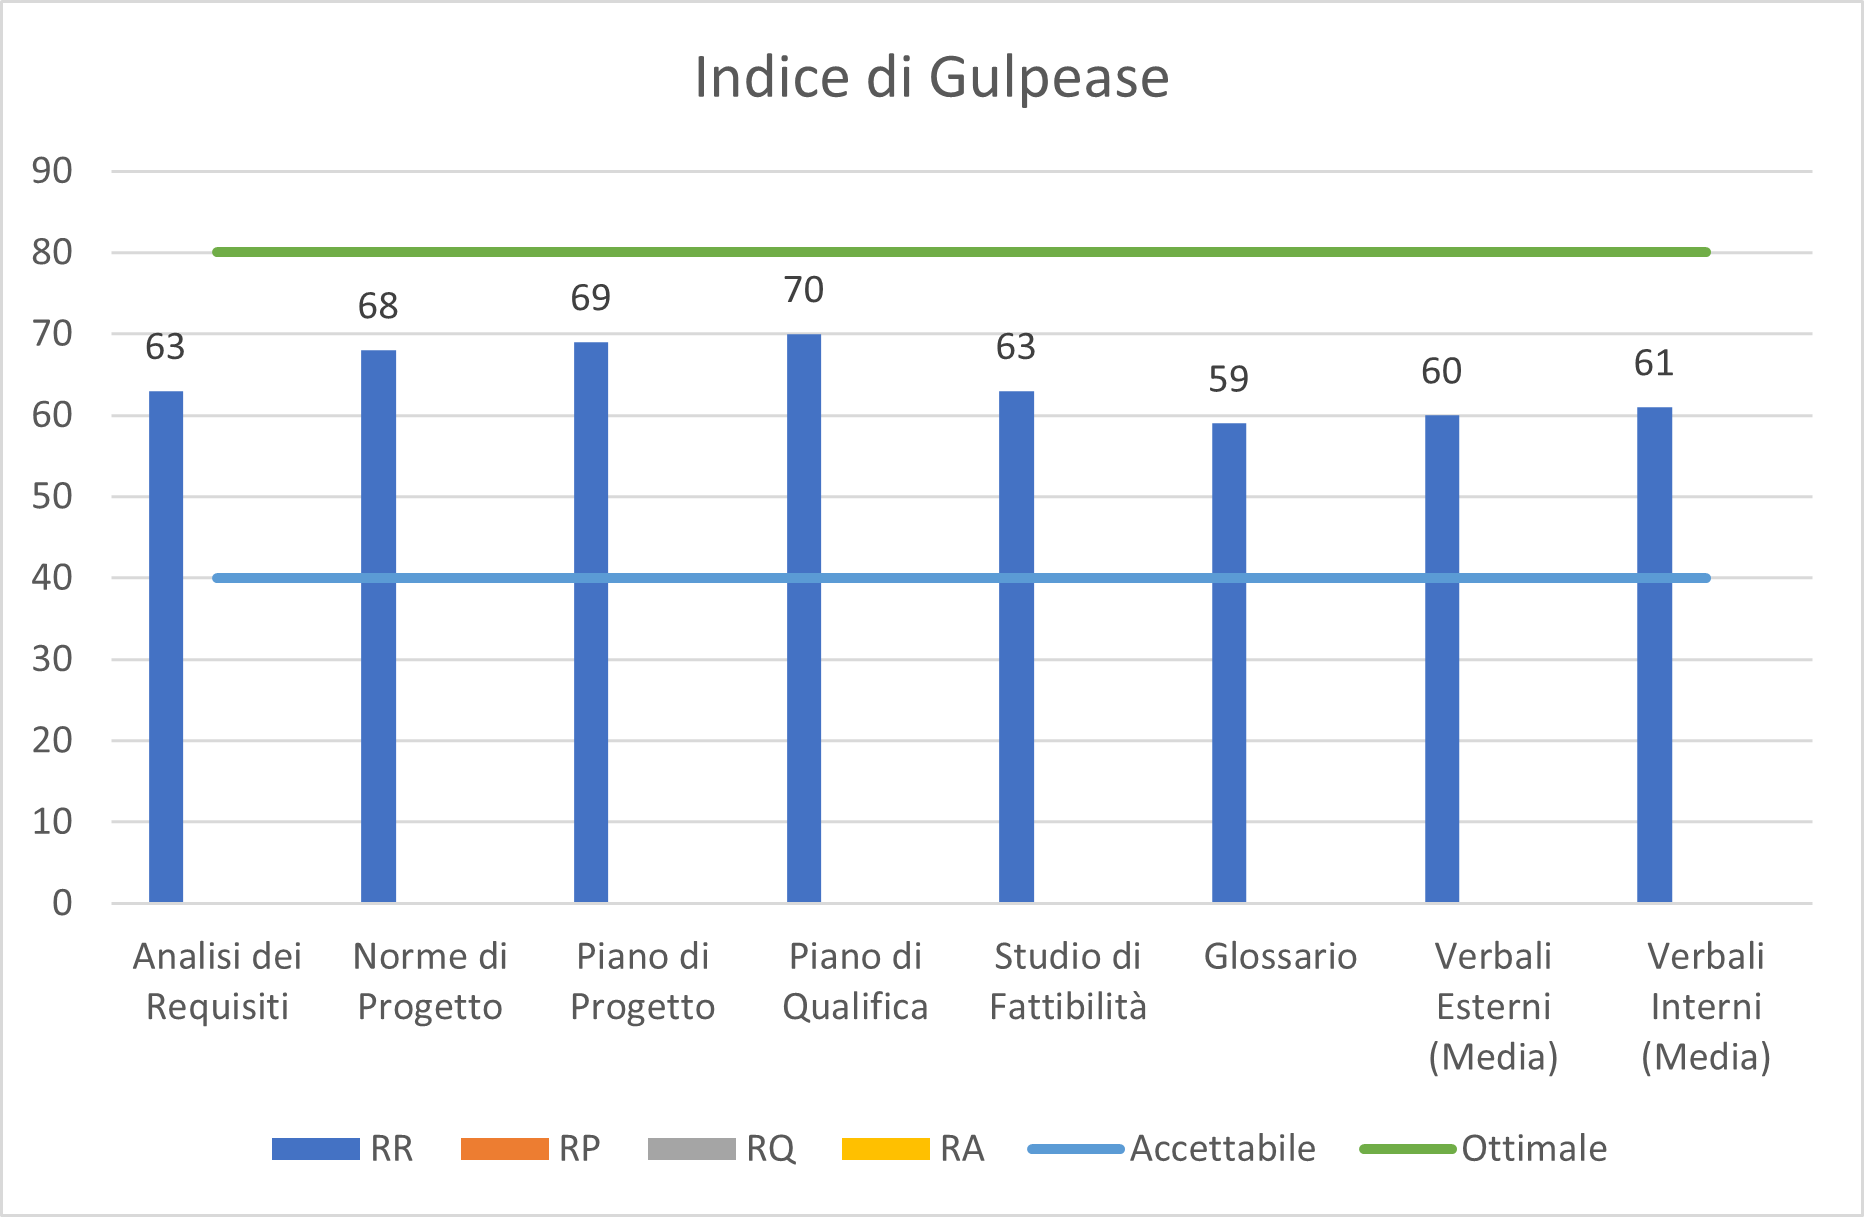
\includegraphics[scale=0.90]{res/ResocontoAttivitaDiVerifica/res/img/indiceGulpease.png}\\
\caption{Andamento complessivo dell'indice di Gulpease}
\end{figure}

\subsubsection{Grafico per documento}

\begin{figure}[H]
\centering
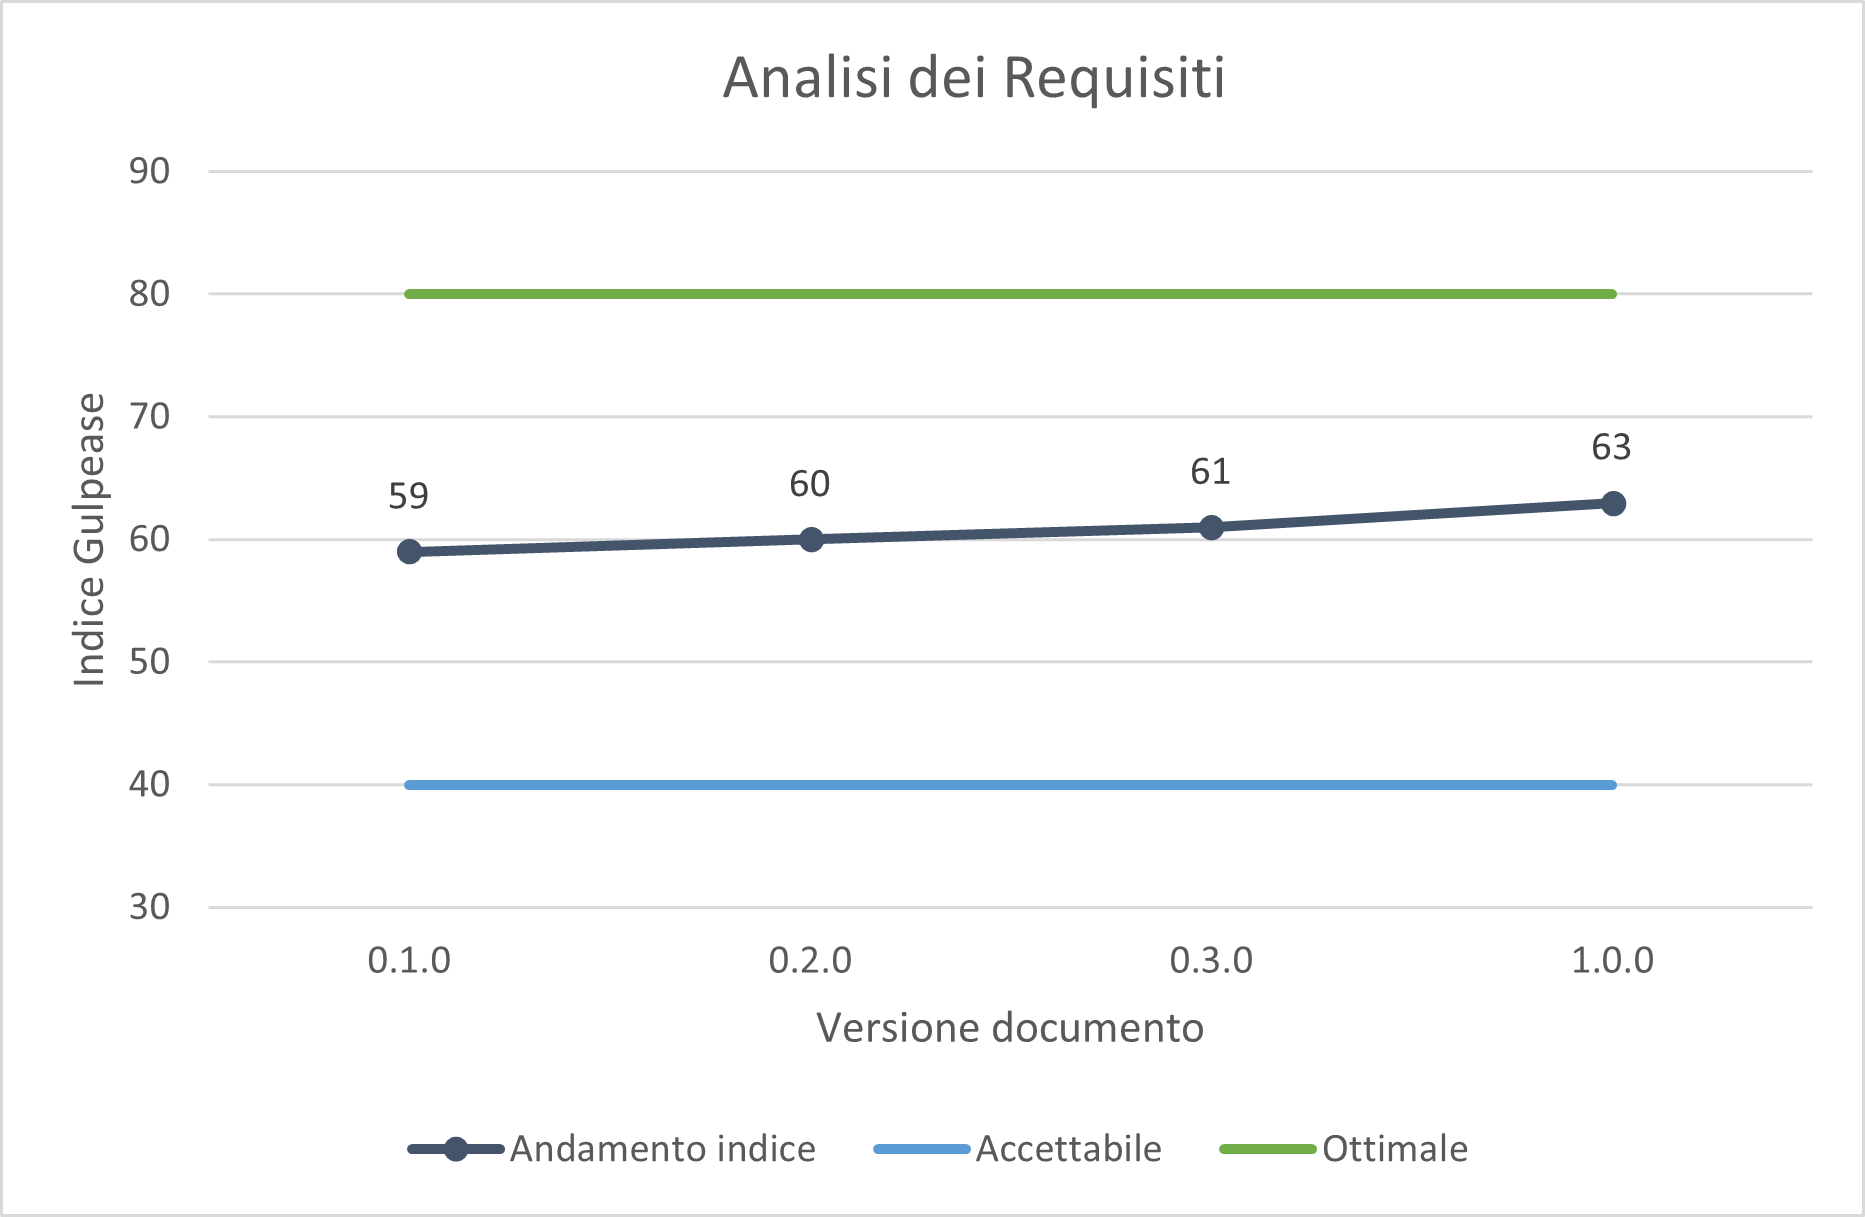
\includegraphics[scale=0.90]{res/ResocontoAttivitaDiVerifica/res/img/gulpeaseADR.png}\\
\caption{Andamento dell'indice di Gulpease \AdR}
\end{figure}

\begin{figure}[H]
\centering
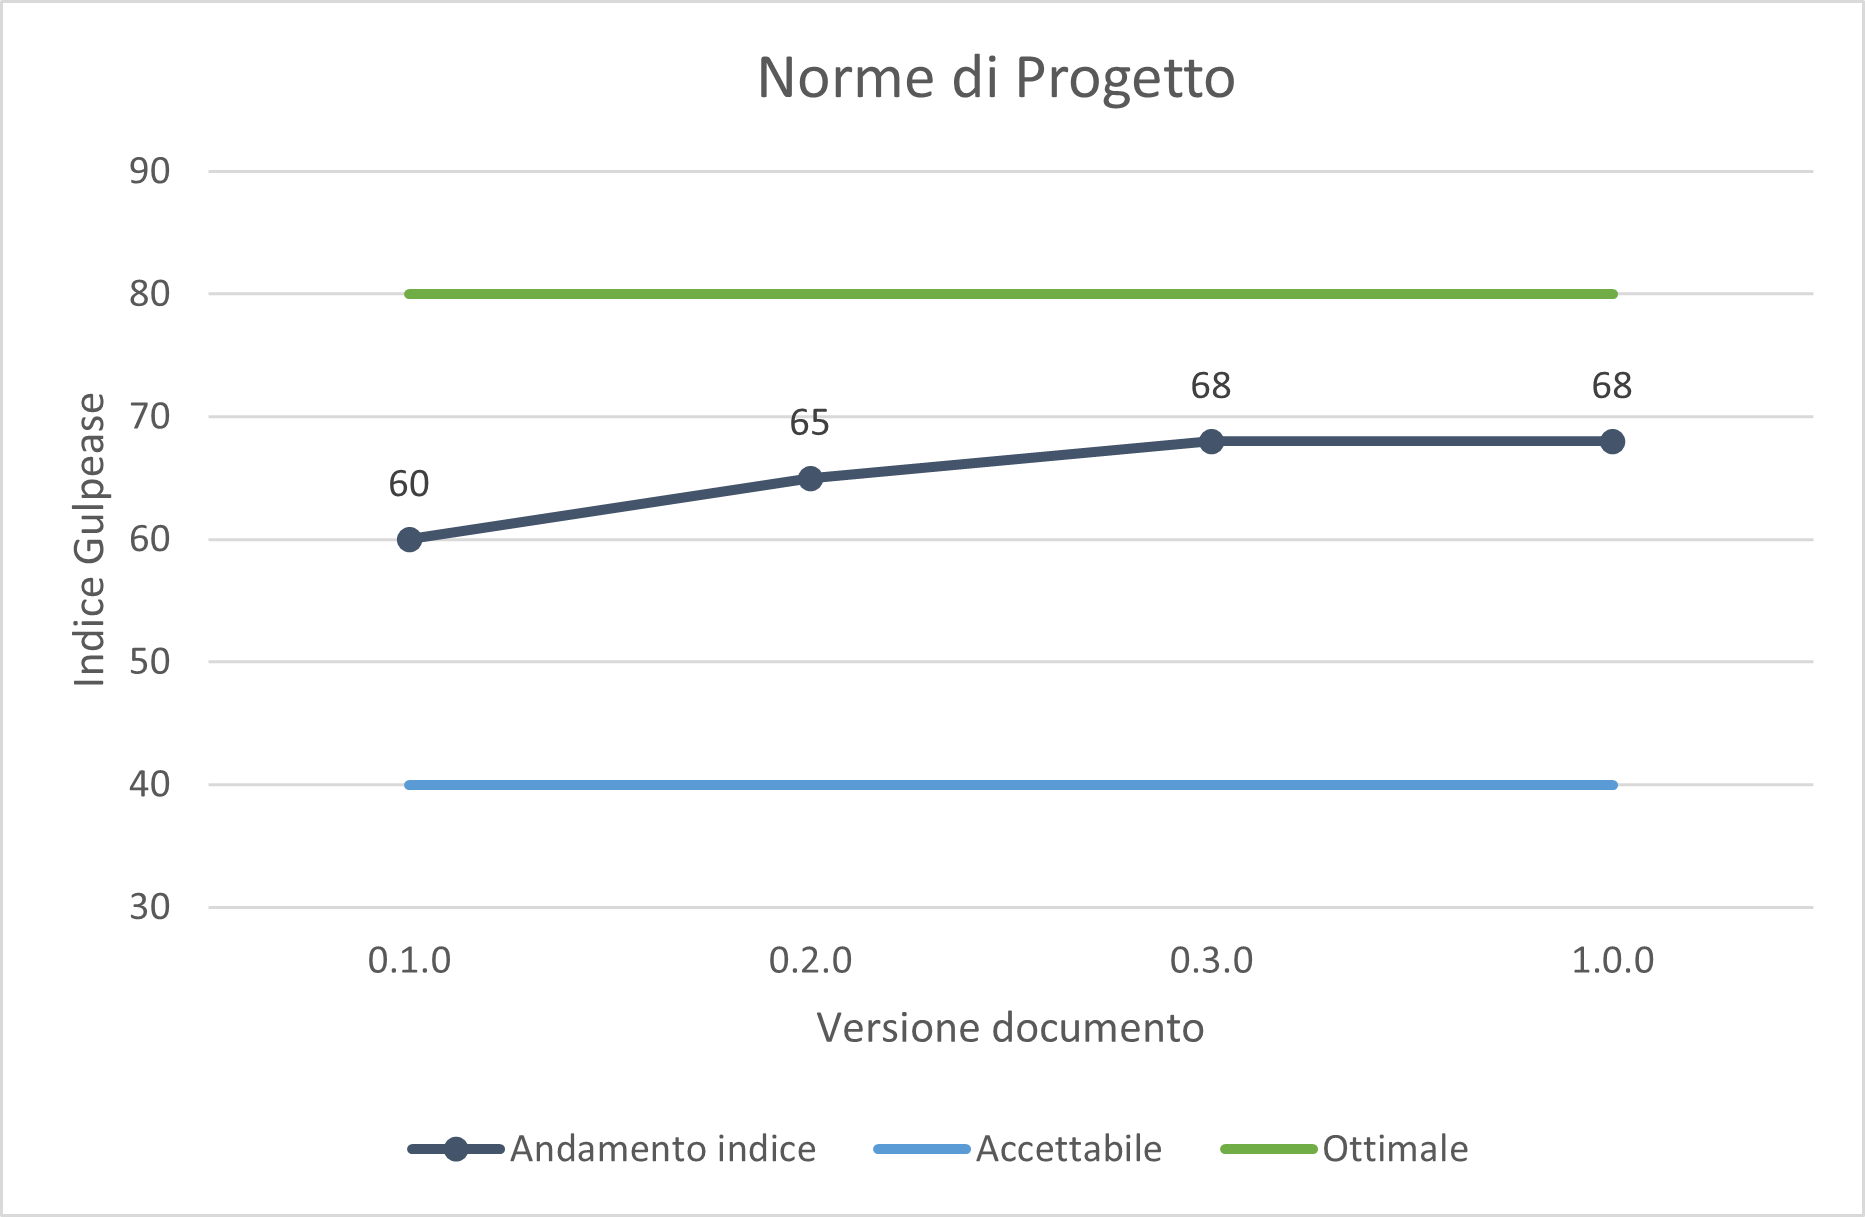
\includegraphics[scale=0.90]{res/ResocontoAttivitaDiVerifica/res/img/gulpeaseNDP.png}\\
\caption{Andamento dell'indice di Gulpease \NdP}
\end{figure}

\begin{figure}[H]
\centering
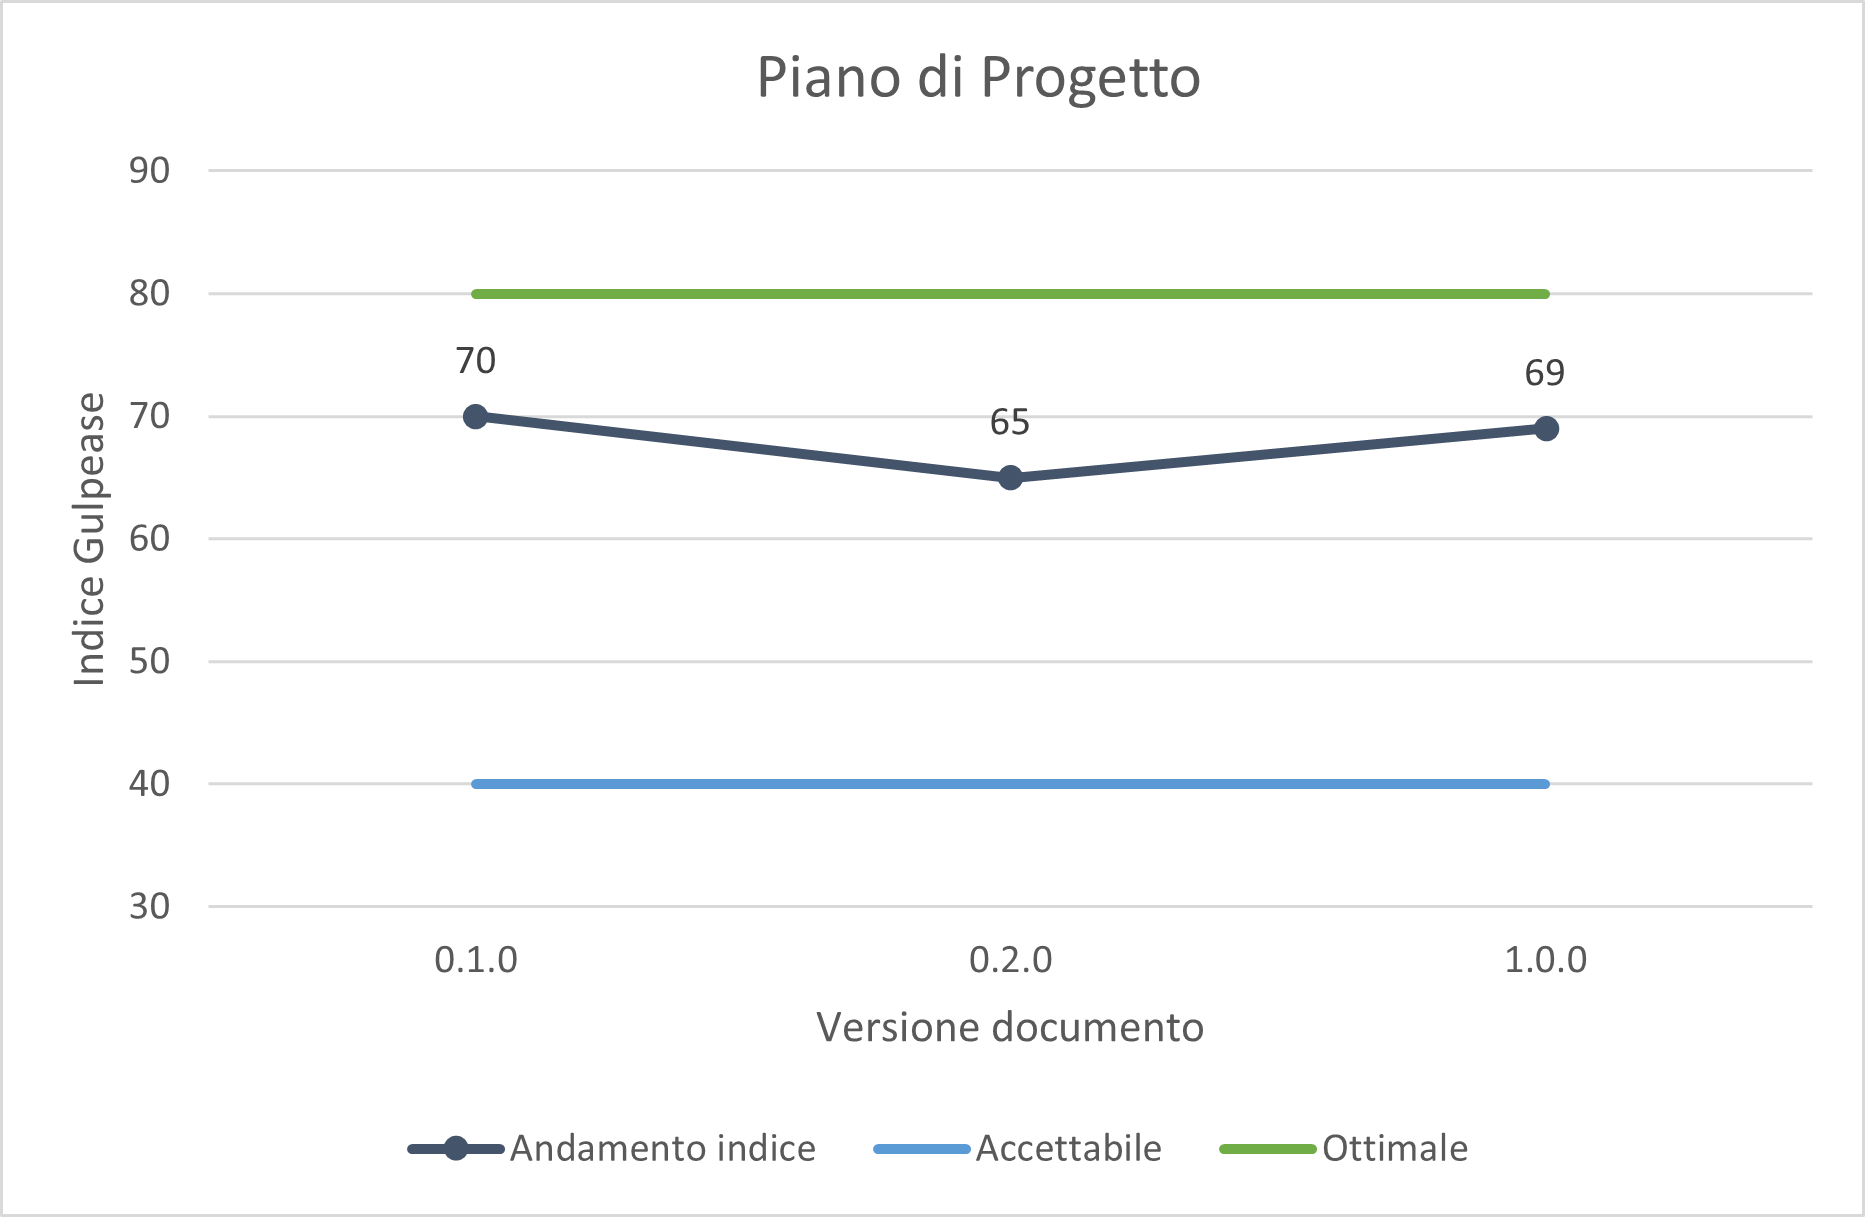
\includegraphics[scale=0.90]{res/ResocontoAttivitaDiVerifica/res/img/gulpeasePDP.png}\\
\caption{Andamento dell'indice di Gulpease \PdP}
\end{figure}

\begin{figure}[H]
\centering
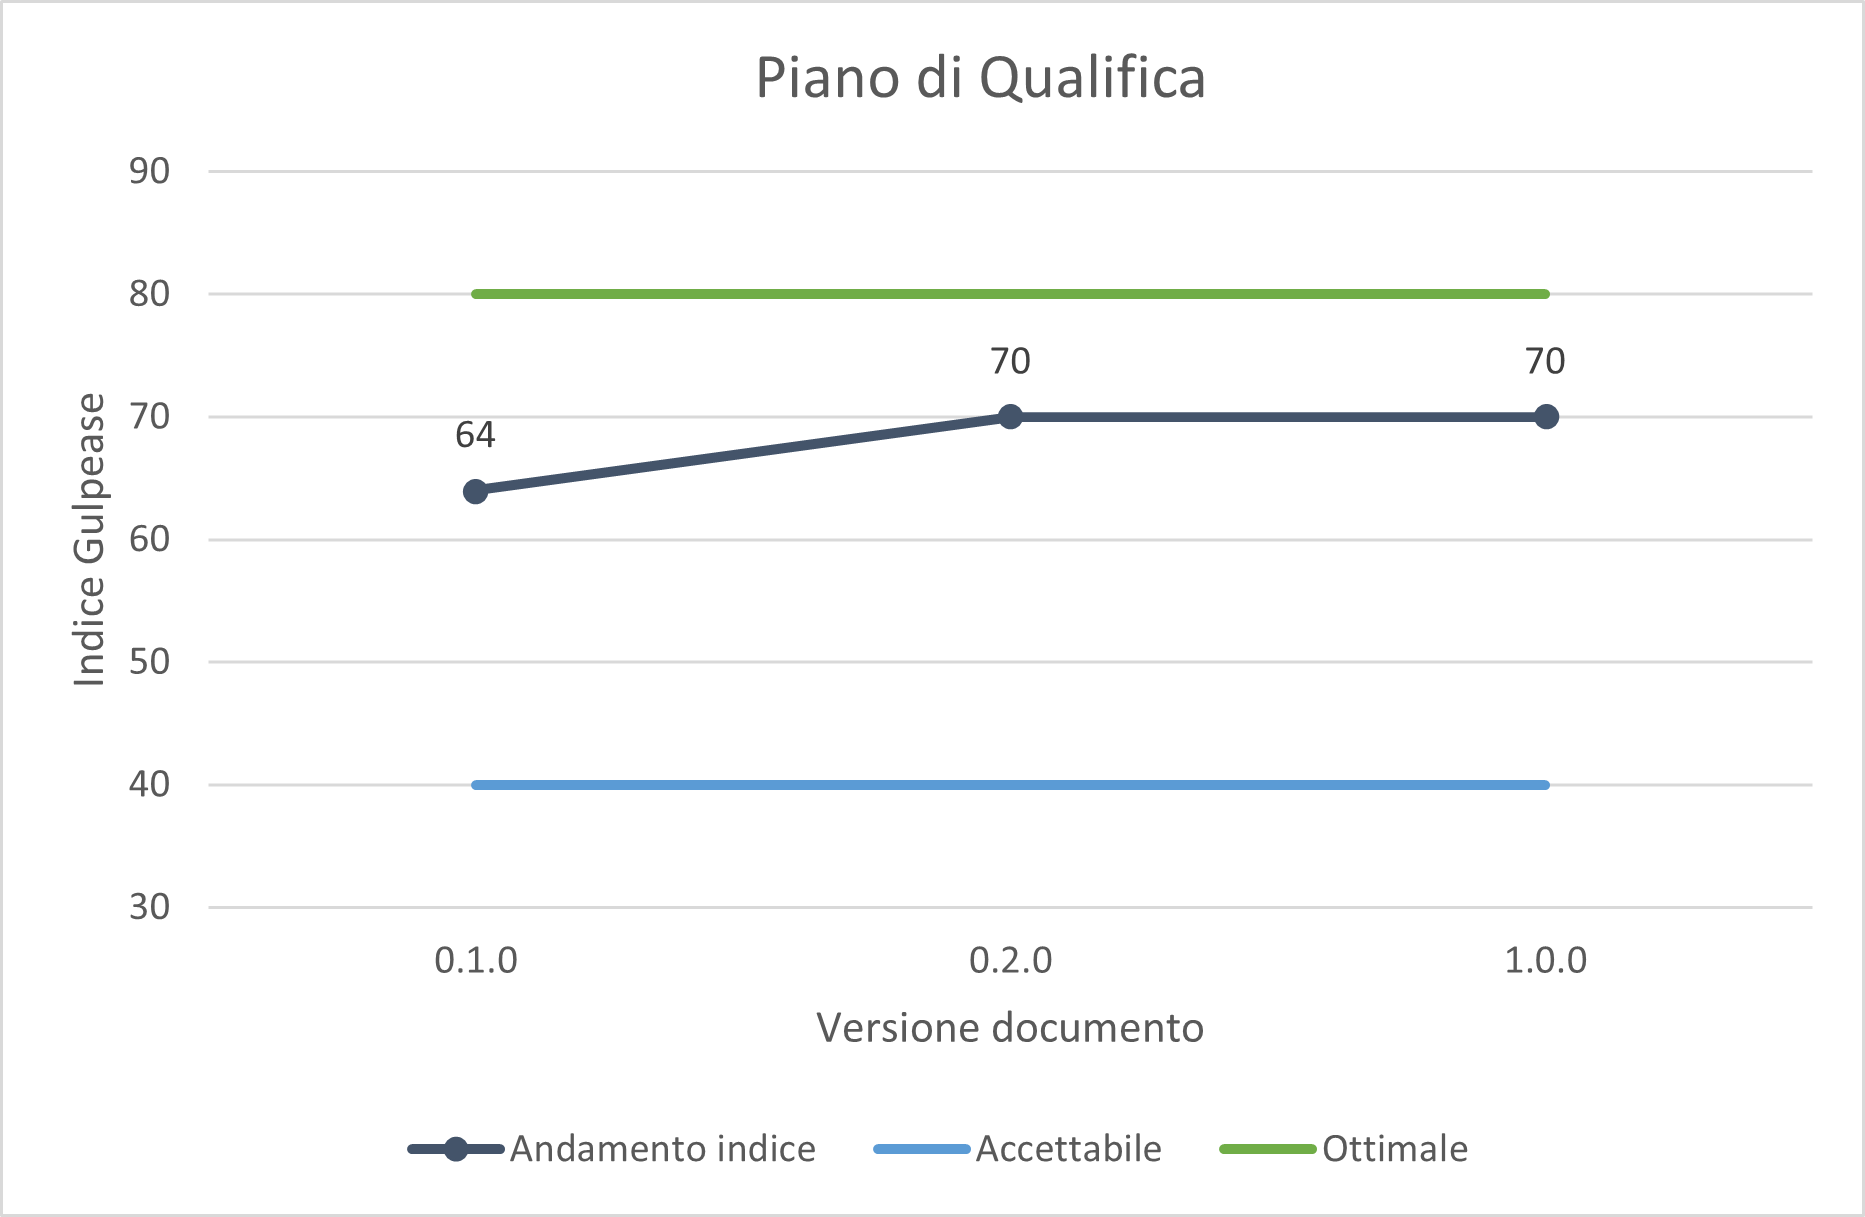
\includegraphics[scale=0.90]{res/ResocontoAttivitaDiVerifica/res/img/gulpeasePDQ.png}\\
\caption{Andamento dell'indice di Gulpease \PdQ}
\end{figure}

\begin{figure}[H]
\centering
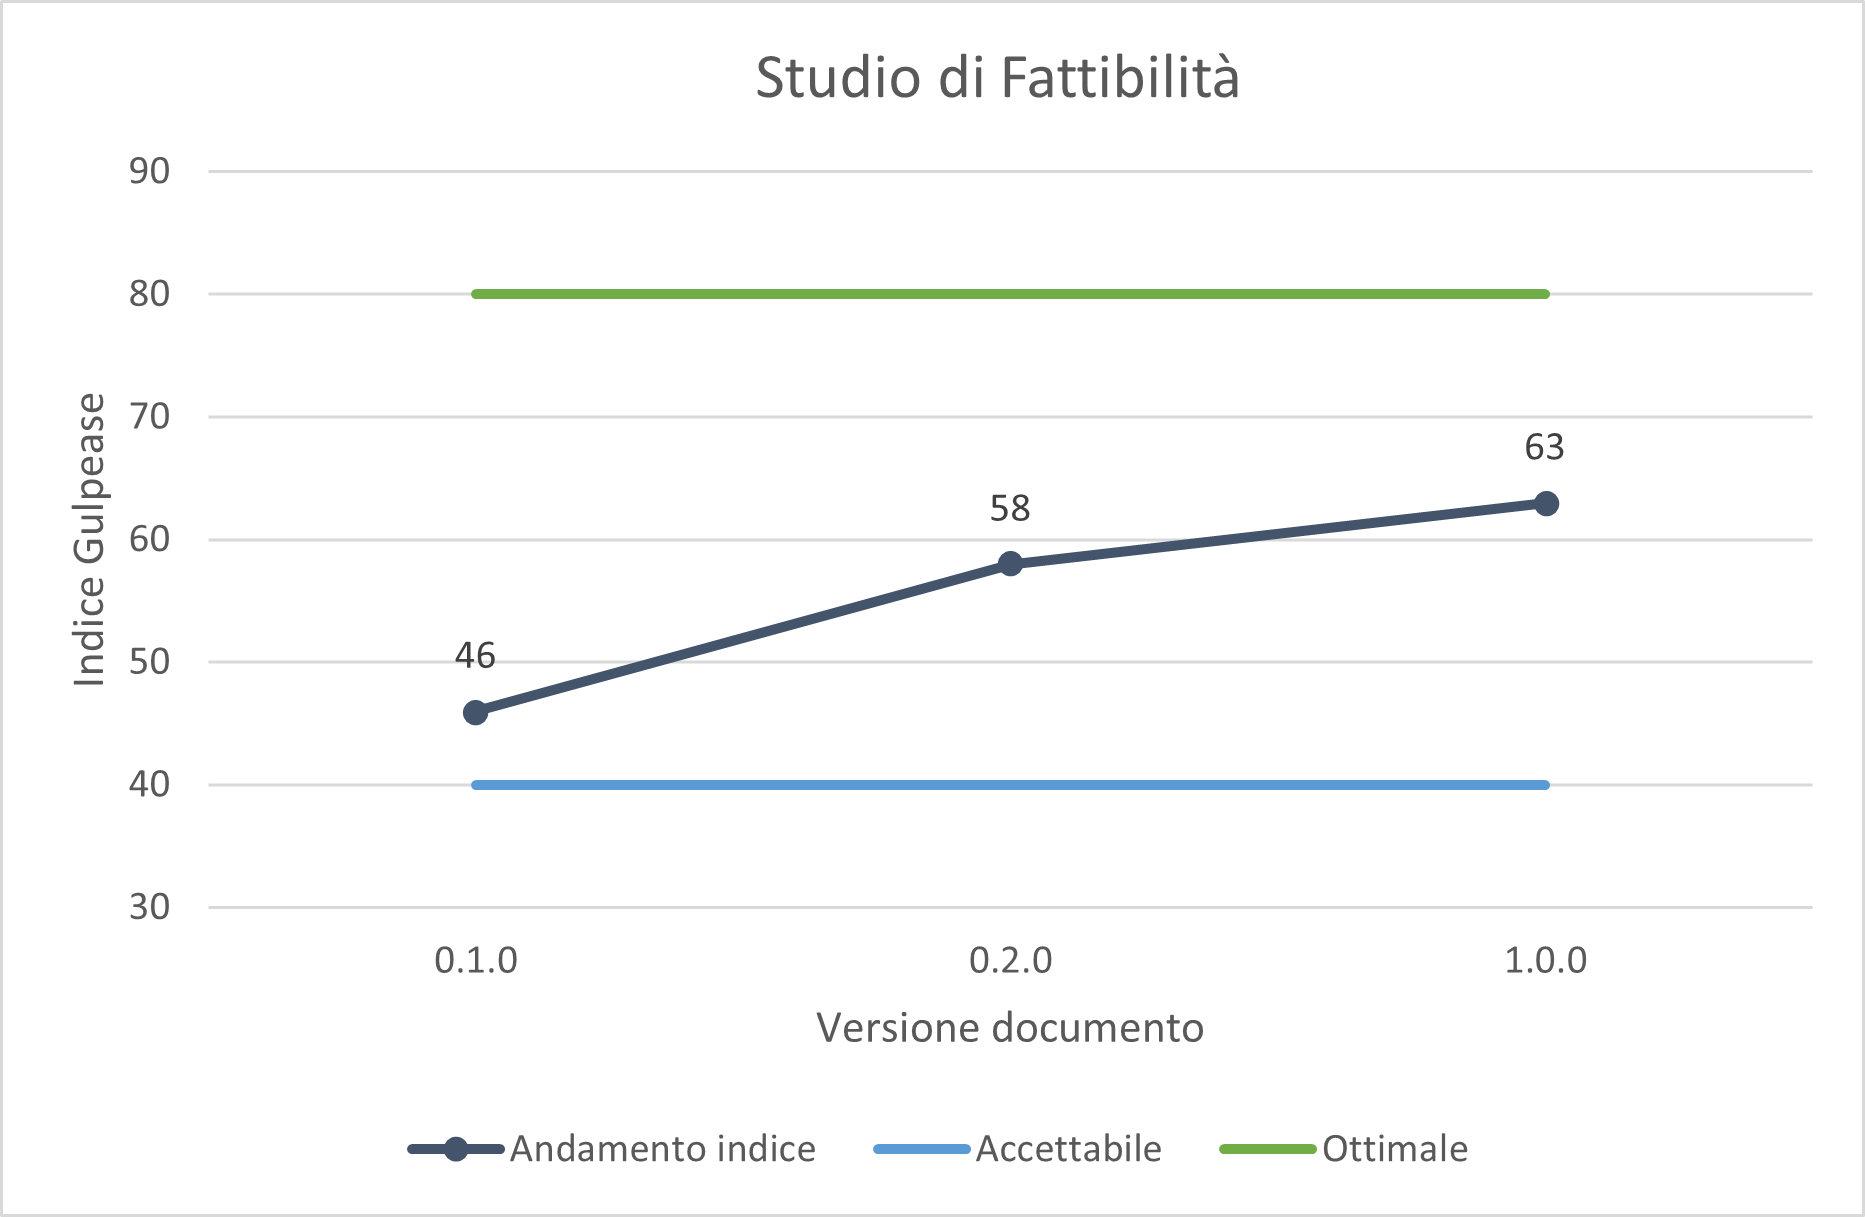
\includegraphics[scale=0.90]{res/ResocontoAttivitaDiVerifica/res/img/gulpeaseSDF.png}\\
\caption{Andamento dell'indice di Gulpease \SdF}
\end{figure}

\begin{figure}[H]
\centering
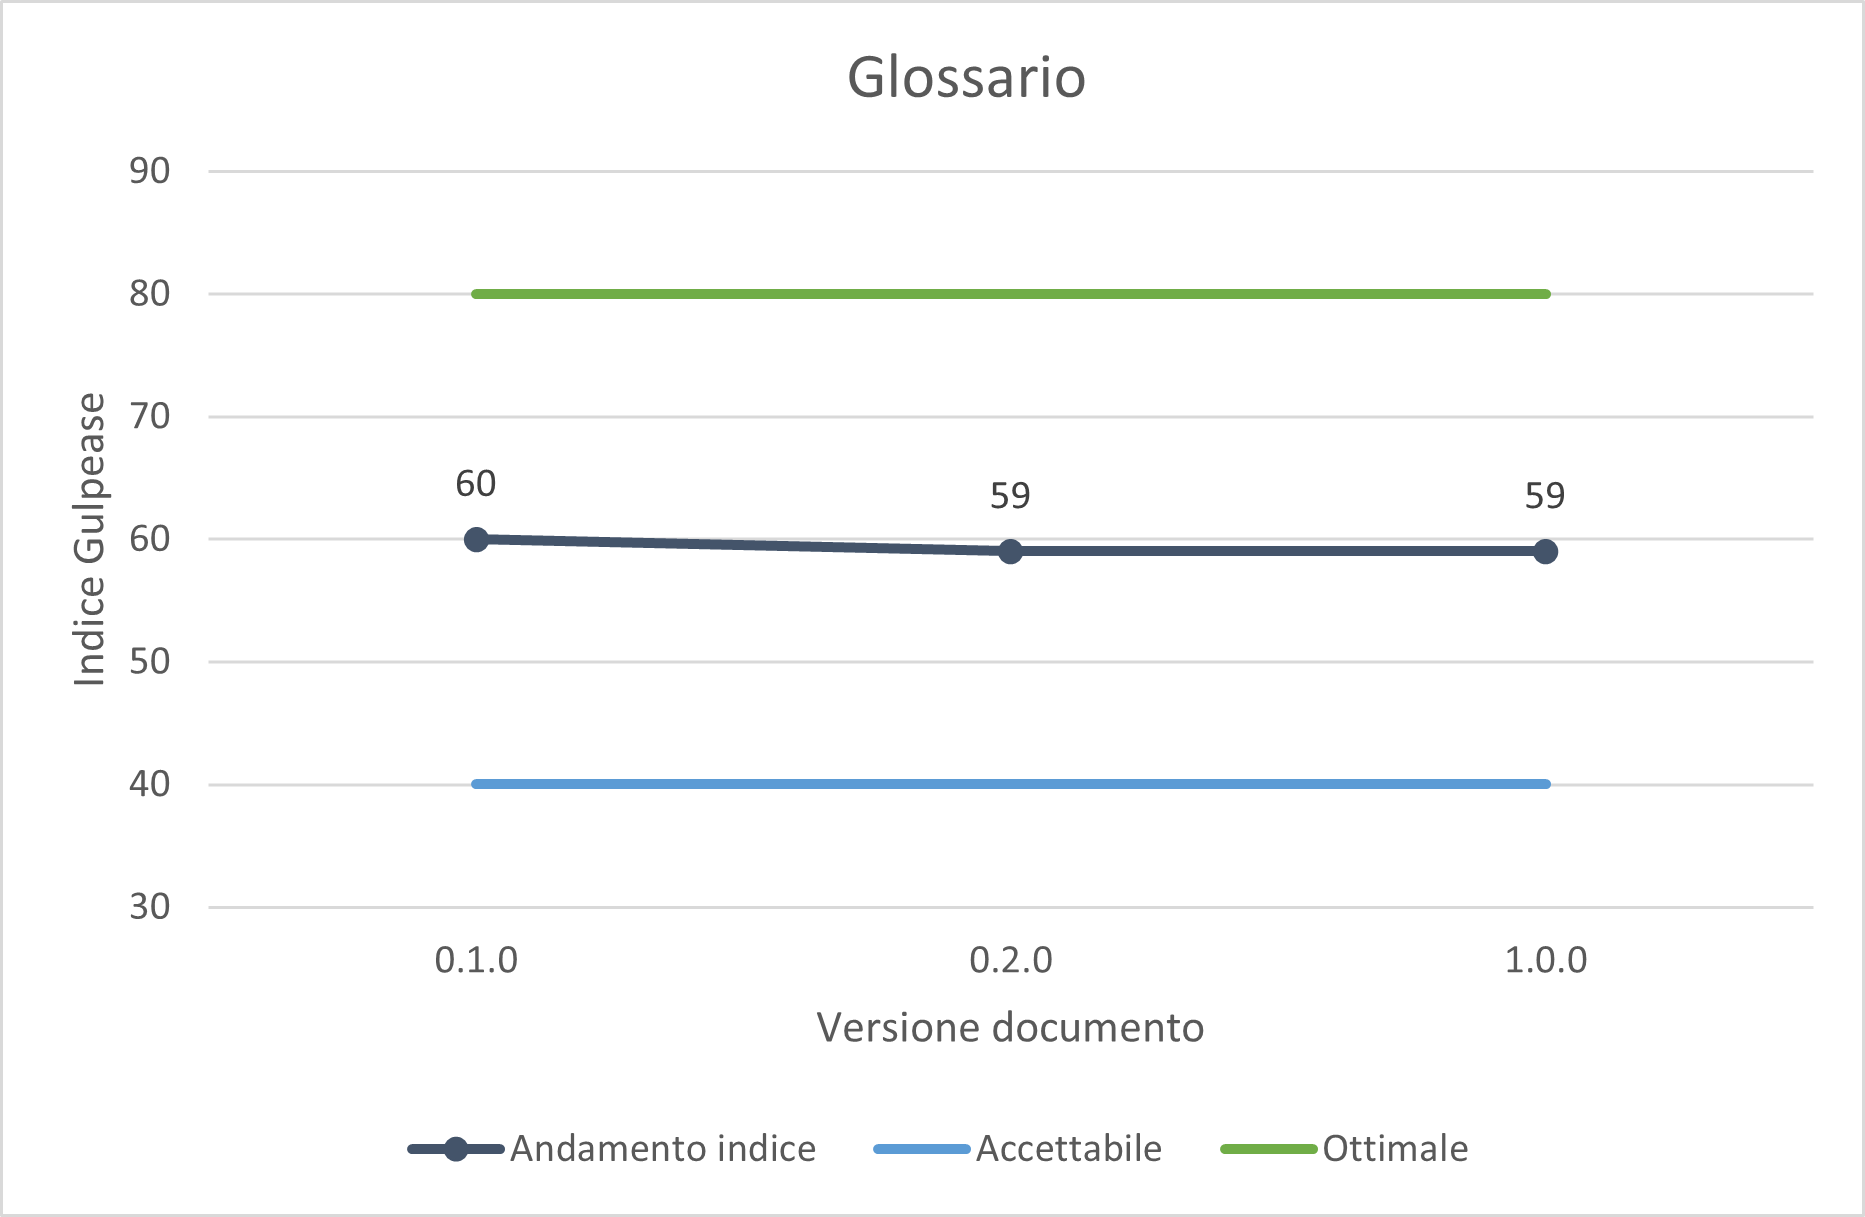
\includegraphics[scale=0.90]{res/ResocontoAttivitaDiVerifica/res/img/gulpeaseG.png}\\
\caption{Andamento dell'indice di Gulpease \Glossario}
\end{figure}

